\documentclass[a4paper,11pt]{report}
\usepackage[T1]{fontenc}
\usepackage[utf8]{inputenc}
\usepackage[polish]{babel}
\usepackage{lmodern}
\usepackage{graphicx}

\title{czas obsługi: tablicy asocjacyjnej}
\author{Tomasz Piotrowski 200524}

\begin{document}
\maketitle
\begin{figure}
\textbf {\Large{ Sprawozdanie z czasu obsługi talbicy asocjacyjnej wykonanej na trzech strukturach:\\
-vektor\\
-drzewo wyszukiwan binarnych\\
-tablica haszujaca\\
. }}
\end{figure}


\begin{figure}
Zmierzony został czas dostepu do elementu w tablicy asocjacyjnej zaimplementowanej na roznych stukturach. Ponieważ czas dostępu do elementu jest bardzo mały funkcja szukajaca elementu wywolana zostala mln razy. Wyniki pomiarow zaprezentowane zostały na wykresie, oraz w tableli
\end{figure}


\begin{figure}

  \begin{center}
	
  
  
    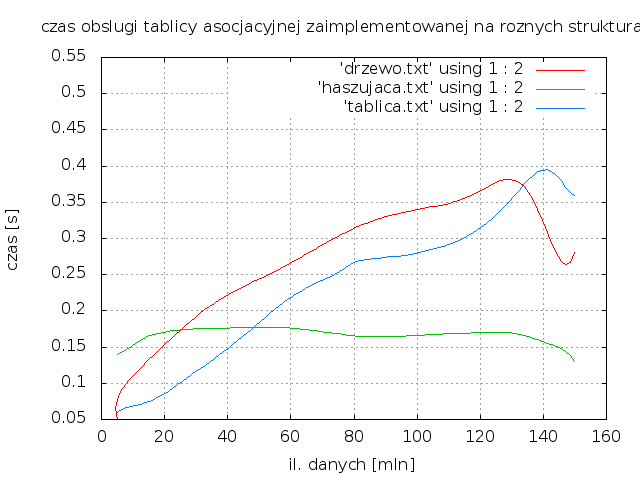
\includegraphics[scale=0.5]{./czas_dzialania_algorytmow.png}
    \label{fig:}
    \caption{}
 
          \begin{tabular}{|l|c|c|r|}
\hline
il[mln] & czas drzewo [s] & haszujaca& vector \\
5.000000 & 0.05& 0.14&0.06\\
1.0000000 &  0.11& 0.14& 0.08\\
15.000000  & 0.11& 0.2&0.06\\
20.000000  & 0.16& 0.16&0.08\\
25.000000  & 0.17& 0.17&0.06\\
30.000000  & 0.22& 0.18& 0.21\\
35.000000 &  0.18& 0.2&0.09\\
40.000000  & 0.24& 0.14&0.09\\
45.000000  & 0.31& 0.19&0.21\\
50.000000  & 0.17& 0.19& 0.21\\
55.000000  & 0.22& 0.15&0.08\\
60.000000  & 0.34& 0.2&0.31\\
65.000000  & 0.22& 0.2& 0.42\\
70.000000  & 0.29& 0.15&0.08\\
75.000000  & 0.35& 0.19&0.11\\
80.000000  & 0.29& 0.14& 0.51\\
85.000000  & 0.35& 0.14&0.22\\
90.000000  & 0.35&  0.17&0.08\\
95.000000  & 0.3& 0.17& 0.38\\
100.000000 &  0.36& 0.18&0.43\\
105.000000 &  0.35& 0.15&0.18\\
110.000000 &  0.36& 0.19&0.1\\
115.000000 &  0.36 & 0.15&0.48\\
120.000000 &  0.24& 0.17&0.11\\
125.000000 &  0.42&  0.17&0.5\\
130.000000 &  0.46&  0.19&0.18\\
135.000000 &  0.48& 0.18&0.47\\
140.000000 &  0.28&  0.13&0.46\\
145.000000 &  0.22& 0.17&0.36\\
150.000000 &  0.28&  0.13&0.36\\
\hline


\hline
\end{tabular}
\newline

   

  \end{center}
\end{figure}

\begin{figure}
    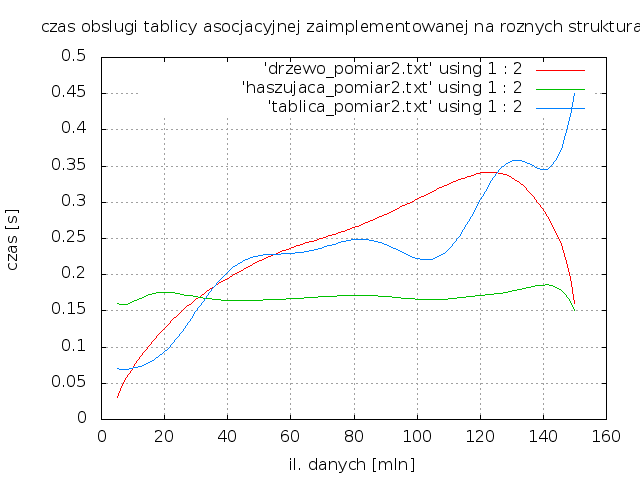
\includegraphics[scale=0.5]{./czas_dzialania_algorytmow2.png}
    \label{fig:}
    \caption{}
         \begin{tabular}{|l|c|c|r|}
\hline
ilosc[mln]&	drzewo&	tablica&	haszujaca\\\hline
5.000000 &	0.03&	0.07&	0.16\\
10.000000&	0.09&	0.06&	0.15\\
15.000000&	0.09&	0.09&	0.18\\
20.000000&	0.14&	0.07&	0.2\\
25.000000&	0.14&	0.08&	0.18\\
30.000000&	0.2&	0.16&	0.16\\
35.000000&	0.19&	0.17&	0.15\\
40.000000&	0.16&	0.26&	0.15\\
45.000000&	0.2&	0.28&	0.18\\
50.000000&	0.26&	0.29&	0.19\\
55.000000&	0.26&	0.08&	0.12\\
60.000000&	0.2&	0.43&	0.18\\
65.000000&	0.25&	0.09&	0.18\\
70.000000&	0.25&	0.08&	0.17\\
75.000000&	0.25&	0.36&	0.14\\
80.000000&	0.3&	0.38&	0.19\\
85.000000&	0.26&	0.17&	0.19\\
90.000000&	0.19&	0.26&	0.2\\
95.000000&	0.36&	0.43&	0.13\\
100.000000&	0.33&	0.09&	0.18\\
105.000000&	0.3&	0.09&	0.13\\
110.000000&	0.32&	0.16&	0.17\\
115.000000&	0.3&	0.17&	0.18\\
120.000000&	0.39&	0.36&	0.17\\
125.000000&	0.37&	0.44&	0.19\\
130.000000&	0.34&	0.46&	0.14\\
135.000000&	0.36&	0.34&	0.19\\
140.000000&	0.25&	0.26&	0.2\\
145.000000&	0.31&	0.34&	0.2\\
150.000000&	0.16&	0.45&	0.15\\

\hline


\hline
\end{tabular}
\end{figure}

\begin{figure}
    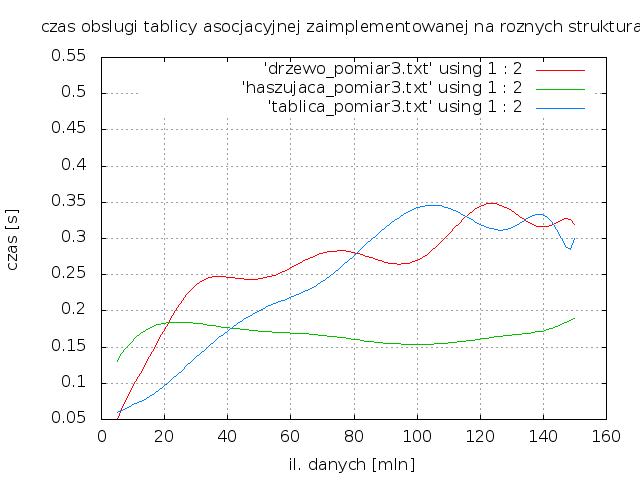
\includegraphics[scale=0.5]{./czas_dzialania_algorytmow3.png}
    \label{fig:}
    \caption{}
       \begin{tabular}{|l|c|c|r|}
\hline
ilosc[mln]&	drzewo[s]&	tablica[s]&	haszujaca[s]\\\hline
5.000000&	0.05&	0.06&	0.13\\
10.000000&	0.1&	0.07&	0.17\\
15.000000&	0.15&	0.08&	0.18\\
20.000000&	0.14&	0.09&	0.2\\
25.000000&	0.21&	0.08&	0.19\\
30.000000&	0.31&	0.17&	0.19\\
35.000000&	0.35&	0.19&	0.16\\
40.000000&	0.2&	0.17&	0.19\\
45.000000&	0.29&	0.09&	0.17\\
50.000000&	0.1&	0.26&	0.17\\
55.000000&	0.22&	0.38&	0.17\\
60.000000&	0.32&	0.06&	0.15\\
65.000000&	0.27&	0.31&	0.18\\
70.000000&	0.25&	0.06&	0.18\\
75.000000&	0.35&	0.36&	0.19\\
80.000000&	0.44&	0.17&	0.14\\
85.000000&	0.15&	0.41&	0.13\\
90.000000&	0.3&	0.37&	0.18\\
95.000000&	0.2&	0.18&	0.13\\
100.000000&	0.2&	0.46&	0.16\\
105.000000&	0.25&	0.38&	0.17\\
110.000000&	0.26&	0.4&	0.13\\
115.000000&	0.37&	0.35&	0.16\\
120.000000&	0.48&	0.27&	0.15\\
125.000000&	0.36&	0.27&	0.18\\
130.000000&	0.33&	0.27&	0.18\\
135.000000&	0.31&	0.28&	0.15\\
140.000000&	0.26&	0.54&	0.17\\
145.000000&	0.36&	0.2&	0.18\\
150.000000&	0.32&	0.3&	0.19\\\hline

\hline
\end{tabular}
\end{figure}
 

\begin{figure}

Wnioski:\\
Na podstawie wykresów można stwierdzić że tablica asocjacyjna zaimplementowana na tablicy haszujacej jest najkorzystniejsza ponieważ czas dostępu do elementu w przybliżeniu jest liniowy O(1). Czas dostępu do elementu wydłuża się w momencie wystąpienia kolizji. I jest on wtedy zależny od ilości. Sytulacja widoczna jest np. na rysumnku 3 dla 20 mln danych.   
\\W przypadku talbiy asocjacyjnej zaimplementowanej na drzewie binarnym oraz na vektorze sortowanym i przeszukiwanym binarnie czas dostepu do szukanego elementu jest podobny. 
Z tabeli można wywnioskować że w przypadku vectora oraz drzewa binarnego czas wyszukiwania zależny jest nie tylko od ilości elementów oraz również od wartości klucza to znaczy od położenie poszukiwanego elementu w całej tablicy, wo wpływa na etap wyszukiwania w którym element zostanie znaleziony.Dobur wyszukiwanego elementu powoduje widoczne zafalowania wartosci funkcji na wykresach. 
\end{figure}

\end{document}
